\section{Introduction}
Tabular data is pervasive in our daily lives, appearing in formats such as databases, scientific articles, web pages, and spreadsheets~\cite{chen2000mining,hurst2000interpretation,hu2023chatdb}. The structured nature of tabular data enables the systematic organization of information into rows and columns, facilitating efficient sorting, querying, and manipulation~\citep{pujara2021tables, chen2020open}. Consequently, table understanding and reasoning have emerged as a significant area of interest in NLP, garnering much attention from researchers~\citep{bao2018table, zhang2024survey}.
% !TEX root = main.tex

\begin{figure}[t]
\vspace{-1.5cm}
\begin{minipage}{0.34\textwidth}
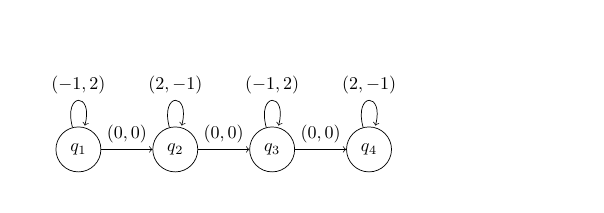
\begin{tikzpicture}[scale=0.25]
\usetikzlibrary{automata, positioning}
\scalebox{0.65}{
\node[state] (q1) {$q_1$};
\node[state, right=of q1] (q2) {$q_2$};
\node[state, right=of q2] (q3) {$q_3$};
\node[state, right=of q3] (q4) {$q_4$};

\path[->] (q1) edge [loop above] node[above] {$(-1,2)$} (q1) edge node[above] {$(0,0)$} (q2); 
\path[->] (q2) edge [loop above] node[above] {$(2,-1)$} (q2) edge node[above] {$(0,0)$} (q3);
\path[->] (q3) edge [loop above] node[above] {$(-1,2)$} (q3) edge node[above] {$(0,0)$} (q4);
\path[->] (q4) edge [loop above] node[above] {$(2,-1)$} (q4);
}
\end{tikzpicture}
\end{minipage}
\begin{minipage}{0.32\textwidth}
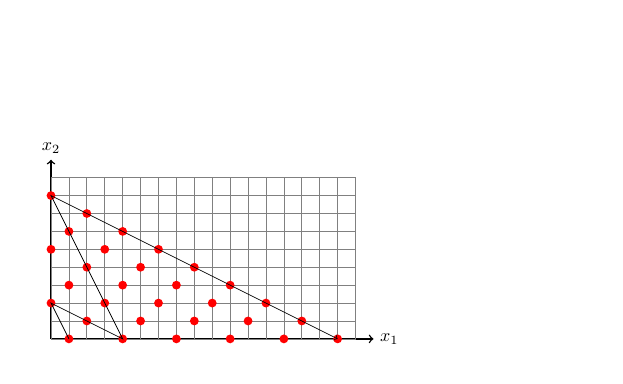
\begin{tikzpicture}[scale=0.35]
\scalebox{0.65}{
\draw[->, thick] (0, 0) -- (18, 0) node[right] {$x_1$};
\draw[->, thick] (0, 0) -- (0, 10) node[above] {$x_2$};

\draw[step=1, gray, thin] (0, 0) grid (17, 9);

\foreach \x in {1,4,7,10,13,16} \fill[red] (\x,0) circle (7pt);
\foreach \x in {2,5,8,11,14} \fill[red] (\x,1) circle (7pt);
\foreach \x in {0,3,6,9,12} \fill[red] (\x,2) circle (7pt);
\foreach \x in {1,4,7,10} \fill[red] (\x,3) circle (7pt);
\foreach \x in {2,5,8} \fill[red] (\x,4) circle (7pt);
\foreach \x in {0,3,6} \fill[red] (\x,5) circle (7pt);
\foreach \x in {1,4} \fill[red] (\x,6) circle (7pt);
\foreach \x in {2} \fill[red] (\x,7) circle (7pt);
\foreach \x in {0} \fill[red] (\x,8) circle (7pt);

\draw[->] (1,0) -- (0,2) -- (2,1) -- (4,0) -- (3,2) -- (2,4) -- (1,6) -- (0,8) -- (2,7) -- (4,6) -- (6,5) -- (8,4) -- (10,3) -- (12,2) -- (14,1) -- (16,0);
}
\end{tikzpicture}
\end{minipage}
\begin{minipage}{0.32\textwidth}
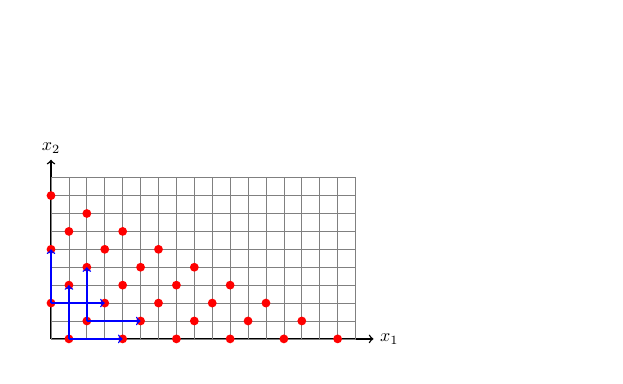
\begin{tikzpicture}[scale=0.35]
\scalebox{0.65}{
\draw[->, thick] (0, 0) -- (18, 0) node[right] {$x_1$};
\draw[->, thick] (0, 0) -- (0, 10) node[above] {$x_2$};

\draw[step=1, gray, thin] (0, 0) grid (17, 9);

\foreach \x in {1,4,7,10,13,16} \fill[red] (\x,0) circle (7pt);
\foreach \x in {2,5,8,11,14} \fill[red] (\x,1) circle (7pt);
\foreach \x in {0,3,6,9,12} \fill[red] (\x,2) circle (7pt);
\foreach \x in {1,4,7,10} \fill[red] (\x,3) circle (7pt);
\foreach \x in {2,5,8} \fill[red] (\x,4) circle (7pt);
\foreach \x in {0,3,6} \fill[red] (\x,5) circle (7pt);
\foreach \x in {1,4} \fill[red] (\x,6) circle (7pt);
\foreach \x in {2} \fill[red] (\x,7) circle (7pt);
\foreach \x in {0} \fill[red] (\x,8) circle (7pt);

\draw[->,blue,thick] (1,0) -- (4,0);
\draw[->,blue,thick] (1,0) -- (1,3);

\draw[->,blue,thick] (2,1) -- (5,1);
\draw[->,blue,thick] (2,1) -- (2,4);

\draw[->,blue,thick] (0,2) -- (3,2);
\draw[->,blue,thick] (0,2) -- (0,5);
}
\end{tikzpicture}
\end{minipage}
\caption{Left: 4-component \dvass $V_2$. 
Middle: the set $\reach_{q_4}(V_2, q_1(1,0))$ and a path $q_1(1,0) \tran q_4(16,0)$.
Right: bases 
%$A = \{(1,0),(2,1),(0,2)\}$ 
and periods 
%$P = \{(0,3),(3,0)\}$
 of an over-approximating semi-linear set $A+P^*$.}
\label{fig:zigzag}
\end{figure}

\begin{example}
For $k\geq 1$, let $V_k$ be a $(2k)$-component \dvass, where each component has just one state $q_i$
and one transition:
$(q_i, (-1,2), q_i)$ for odd $i$, and $(q_i, (2,-1), q_i)$ for even $i$.
Bridge transitions are $(q_i, (0,0), q_{i+1})$.
Figure~\ref{fig:zigzag} shows $V_2$ (left) and 
a path in $V_2$ from $s = q_1(1,0)$ to $t = q_4(16,0)$ together with 
the reachability set $\reach_{q_4}(V_2, s)$ (middle).
In general,
\begin{align} \label{eq:reachk}
X_k := \reach_{q_{2k}}(V_k, s) \ = \ \set{(x_1,x_2) \mid x_1+2x_2 \leq 4^k, \  x_1+2x_2 \equiv 1 \!\! \mod 3}.
\end{align}
Even if the size of the reachability set is 
exponential in $k$, for small $(x_1, x_2)$ it is periodic and the periods are small.
The set $X_k$ can be over-approximated by $A + P^*$ for $A = \set{(1,0),(2,1),(0,2)}$ and $P = \set{(0,3),(3,0)}$
(shown on the right of Figure~\ref{fig:zigzag}), namely for every $k\geq 1$ and $B\in\N$,
the set $X_k$ is \kanapka {$8$} {$B$}. 
For illustration, consider $Y := X_k \cap ((1,0) + P^*)$.
If $(1,0) + P^{\leq B} \subseteq X_k$ then $Y$ is a $B$-approximation
of $(1,0) + P^*$ with $\norm((1,0)), \norm(P) \leq 3 \leq 8$. 
Otherwise, there is some $(v_1, v_2) \in \big((1,0) + P^{\leq B}\big)\setminus X_k$, and
then $B$ is larger than $4^k$:
\[
%8B \geq 2(1 + 3B) \geq 2(v_1 + v_2) \geq v_1 + 2 v_2 > 
4^k < v_1 + 2 v_2 \leq 2(v_1 + v_2) \leq 2(1+3B) \leq 8B.
\]
Therefore by \eqref{eq:reachk}, each $(x_1,x_2) \in Y$ satisfies 
$\norm(x_1,x_2) = x_1 + x_2 \leq x_1 + 2x_2 \leq 4^k < 8B$, and thus
$Y$, seen as a union of singletons, is a union of 
linear sets with norm of base bounded by $8B$ and empty set of periods. 
In both cases, 
$Y$ is \kanapka {$8$} {$B$}. 
%The same intuition stays behind polynomial approximability of \dvass stated in Lemma~\ref{lem:2vass-sandwich}.
\end{example}

Thrived on the logical reasoning capabilities of Large Language Models (LLMs), using LLMs for dealing with table-related tasks has become a mainstream research direction~\cite{chen2023large,zhang2024survey,dong2024large}. Existing table understanding methods convert tables into linear text sequences and focus on designing prompts or instructions to stimulate LLMs to conduct effective reasoning over tables~\cite{chen2023large,wang2024chainoftable}. However, they typically provide a fixed text representation of the tabular format for reasoning. Recent studies have also shown that LLMs are sensitive to the text representation of tables~\cite{liu-etal-2024-rethinking}, motivating researchers to explore the most suitable text-based tabular formats for different table understanding scenarios~\cite{zhang2024flextaf,sui2024table,singha2023tabular}.


Besides text-based table representations, many works use the screenshot of table as its image-based representation during reasoning to explore the effectiveness of Multi-modal Large Language Models (MLLMs) in understanding table images~\cite{deng2024tables,ZhengFSS0J024}. As shown in Figure~\ref{fig:example}, both text-based and image-based table representations potentially play distinct roles in enhancing the table reasoning abilities of MLLMs. Specifically, in the first case, the question asks, ``What is the total number of wins listed for the United States?'', which requires the model to identify the wins of the United States, namely ``18'', ``2'' and ``2'', and then sum them to obtain the correct answer, ``22''. The text-based table representation enables LLMs to produce the correct answer because the question relies more on the arithmetic ability of language models. In contrast, the image-based table representation allows MLLMs to correctly answer the question in the second case. This is enabled by the visual annotation of teams with different colors to represent the win-loss situation. Both the color and cell position in the image provide crucial semantics to help MLLMs accurately answer the question. Despite these advantages, existing works~\cite{deng2024tables,ZhengFSS0J024} mainly focus on investigating the table understanding capabilities of MLLMs using unimodal representations, leaving room for further exploration of multi-modal representations to enable more effective table reasoning.

This paper introduces the \textbf{H}ybr\textbf{I}d-modal \textbf{P}reference o\textbf{P}timizati\textbf{O}n (\method{}) model, which integrates both text-based and image-based table representations for enhancing the table understanding capability of MLLMs. Specifically, \method{} proposes a Hybrid-Modal Preference Optimization method to guide MLLMs in answering questions by leveraging more comprehensive information from different modalities of table representations. \method{} prompts the MLLM to generate responses based on both unimodal and multi-modal representations of the table. Then, it selects the most representative negative responses using the self-consistency~\cite{liu-etal-2024-rethinking} of MLLMs when answering questions based on different modalities, thereby mitigating unnecessary modality bias during training. These negative responses are subsequently collected to optimize the MLLMs using the DPO method~\cite{rafailov2023direct}, helping the model to assign higher probabilities to ground truth answers over negative responses.

Our experiments demonstrate the effectiveness of our \method{} model by achieving more than a 4\% improvement over different table understanding models, which underscores the importance of incorporating both text-based and image-based representations in table understanding tasks. Additionally, \method{} significantly enhances the performance of MLLMs even with unimodal table representations, illustrating the generalization ability of our training method. Our further analyses show that \method{} optimizes MLLMs to better extract semantic information, generate more consistent answers, and engage in diverse reasoning processes based on table representations of different modalities, thereby enabling more accurate predictions based on multi-modal table representations.